\chapter{Auswertung Benchmark}
In dem vorgenommenen Benchmark wurden alle Queries 250 mal wiederholt.
Im folgenden werden die Ergebnisse des Benchmarks ausgewertet.
Dazu wird zu erst die Gesamtlaufzeit des Benchmarks in \autoref{auswertung:generell} analysiert. Dabei wird zwischen zeilenbasierten und spatenbasierten
Tabellen unterschieden.
Anschließend wird in \autoref{auswertung:queries} auf die Laufzeit der
einzelnen Unterabfragen des Benchmarks eingegangen.
Dabei soll untersucht werden welche Abfragen besonders schnell sind.
In \autoref{auswertung:basic_indizes} und \autoref{auswertung:hardware}
wird der Einfluss von Indizes bzw.\ unterschiedlicher Hardwarekonfigurationen
untersucht.

\section{Gesamtlaufzeit des Benchmarks}\label{auswertung:generell}


Allgemein sollten Benchmarks auf der HANA Datenbank immer zwischen
Row- und Columnstore unterscheiden.
Dies wird deutlich beim Betrachten der Allgemeinen Laufzeit.
Wie \autoref{auswertung:gesamtlaufzeit} zu entnehmen ist, besteht ein deutlicher
Unterschied in der Laufzeit zwischen Row- und Columnstore.
Der Columnstore ist im Durschnitt um 79\% schneller.

\begin{tabularx}{\textwidth}{Xrr}
	\toprule
	 & \textbf{Columnstore} & \textbf{Rowstore}\\
	\midrule
	\endhead
	\hline
	\caption{Gesamtlaufzeiten von Row- und Columnstore in msec mit 250 Wiederholungen}
	\label{auswertung:gesamtlaufzeit}
	\endfoot
	Durchschnitt & 371 & 1727 \\
	Minimum & 359 & 1645 \\
	Maximum & 488 & 1902 \\
	Median & 369 & 1722 \\
	Standardabweichung & 12 & 40\\
	Gesamt & 92855 & 431635 \\
\end{tabularx}

Da der SSBM Benchmark als Maß für Abfragen im Bereich des Datawarehouse
eingesetzt wird, kann also allgemein gesagt werden,  dass der Columnstore
dem Rowstore im Datawarehouse Umfeld vorzuziehen ist.
Jedoch sollte bedacht werden, dass es sich bei dem SSBM Benchmark um
reine Abfragen von Daten handelt. Wie in \autoref{row_col:rowstore} beschrieben
kann ein Rowstore von Vorteil sein, wenn Daten gespeichert werden.

\begin{figure}[H]
	\centering
	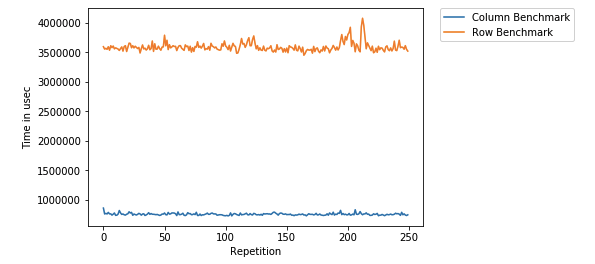
\includegraphics[width=0.7\textwidth]{images/performanceentwicklung.png}
	\caption{Gesamtlaufzeit von Row- und Columnstore}\label{auswertung:gesamtlaufzeit:graph}
\end{figure}
Anhand der Standardabweichung und \autoref{auswertung:gesamtlaufzeit:graph} ist auch zu sehen, dass der Columnstore
eine konstantere Zeit pro Abfrage aufweist.
Allerdings da der Rowstore im allgemeinen langsamer ist als der Columnstore
kann dies vernachlässigt werden, da die Standardabweichung relativ zur
Gesamtlaufzeit sehr gering ist.

\section{Vergleich der SSBM Queries}\label{auswertung:queries}

Im folgenden wird die Laufzeit einzelner Queries des SSBM Benchmarks separat betrachtet.
Dazu wird der Benchmark in die Gruppen Q1, Q2, Q3 und Q4 unterteilt.
Diese Gruppen bestehen aus einzelnen Unterabfragen Q1.1, Q1.2 etc.
Zuerst wird allgemein die Geschwindigkeit der einzelnen Gruppen verglichen
und anschließend auf ausgewählte Unterabfragen eingegangen.

\newcolumntype{f}{>{\columncolor{yellow}}r}
\newcolumntype{s}{>{\columncolor{red}}r}

\begin{table}[H]
	\resizebox{\textwidth}{!}{%
	\begin{tabular}{l|rfrr|rrrs}
		\toprule
		 & \multicolumn{4}{c|}{Columnstore} & \multicolumn{4}{c}{Rowstore} \\
		 & \textbf{Q1} & \textbf{Q2} & \textbf{Q3} & \textbf{Q4} & \textbf{Q1} & \textbf{Q2} & \textbf{Q3} & \textbf{Q4}\\
		\midrule
		Durchschnitt & 103,5 & 61,5 & 95,0 & 111,3 & 414,0 & 345,4 & 477,6 & 489,5\\
		Median & 101,9 & 60,2 & 93,6 & 109,6 & 412,8 & 343,2 & 474,9 & 485,9\\
		Maximum & 160,1 & 90,7 & 111,2 & 143,7 & 497,4 & 415,5 & 579,7 & 562,6\\
		Minimum & 100,3 & 58,3 & 91,4 & 106,3 & 385,6 & 311,1 & 441,5 & 454,0\\
		Standardabweichung & 5,7 & 3,9 & 3,5 & 5,0 & 2 & 15,9 & 17,7 & 17,2\\
		Gesamt & 25884,6 & 15385,1 & 23748,9 & 27836,4 & 103507,9 & 86354,2 & 119398,3 & 122374,7\\
	\end{tabular}%
	}
	\caption{Laufzeit: Q1-4 von Row- und Columnstore in msec mit 250 Wiederholungen}
	\label{auswertung:queries-overview}
\end{table}

Wie in \autoref{auswertung:queries-overview} zu sehen ist,
ist die schnellste Query mit einer Durchschnittlaufzeit von 61,5 msec Q2 des Columnstores,
wohingegen Q4 des Rowstores die langsamste Query mit einer Durchschnittlaufzeit von
489 msec ist.

Im folgenden soll verglichen werden welche Queries die größte Verbesserung durch
Verwendung des Columnstores aufweisen.
Dazu wird die Durchschnittlaufzeit aller einzelnen Subqueries Q1.1-Q4.3
zwischen Row- und Columnstore verglichen und der relative Performanzgewinn errechnet.

\begin{table}[H]
	\resizebox{\textwidth}{!}{%
	\begin{tabular}{l|rrrrrrrrrrrrr}
		\toprule
		 & \textbf{Q1.1} & \textbf{Q1.2} & \textbf{Q1.3} & \textbf{Q2.1} & \textbf{Q2.2} & \textbf{Q2.3} & \textbf{Q3.1} & \textbf{Q3.2} & \textbf{Q3.3} & \textbf{Q3.4} & \textbf{Q4.1} & \textbf{Q4.2} & \textbf{Q4.3}\\
		\midrule
		Rowstore & 163,56 & 126,25 & 124,69 & 134,93 & 108,39 & 99,14 & 186,91 & 113,75 & 85,76 & 87,23 & 196,88 & 162,72 & 123,76\\
		Columnstore  & 35,95 & 47,0 & 21,29 & 28,03 & 25,63 & 7,92 & 31,19 & 23,34 & 21,01 & 20,61 & 47,06 & 42,8 & 22,29\\
		Difference  & 127,61 & 79,25 & 103,4 & 106,9 & 82,76 & 91,22 & 155,72 & 90,41 & 64,75 & 66,61 & 149,82 & 119,93 & 101,47\\
		in \% & 78,0 & \cellcolor{red} 62,8 & 82,9 & 79,2 & 76,4 & \cellcolor{yellow} 92,0 & 83,3 & 79,5 & 75,5 & 76,4 & 76,1 & 73,7 & 82,0\\
	\end{tabular}%
	}
	\caption{Vergleich Row- vs. Columnstore von Q1.1-Q4.3 in msec mit 250 Wiederholungen}
	\label{auswertung:row-vs-column}
\end{table}

Wie aus \autoref{auswertung:row-vs-column} zu entnehmen ist hat Q2.3 die größte
Performanzsteigerung von 92 \%.
Im Gegensatz dazu hat Q1.2 die geringste Performanzsteigerung und liegt dabei unter
der durchschnittlichen Performanzsteigerung von 78,29\%.

\begin{figure}[H]
	\centering
	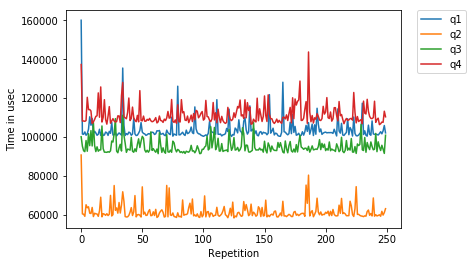
\includegraphics[width=0.49\textwidth]{images/Analysis-SSBM-HANA_18_0.png}
	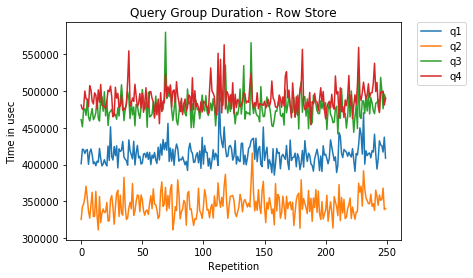
\includegraphics[width=0.49\textwidth]{images/Analysis-SSBM-HANA_23_0.png}
	\caption{Query-Gruppen Laufzeit}\label{auswertung:query-group}
\end{figure}

In \autoref{auswertung:query-group} ist zu erkennen, dass die
Laufzeit einzelner Queries durch zeilenbasiete bzw.\ spaltenbasierte
Tabellen beeinflusst wird. Zwar sind allgemein die spaltenorientierten Tabellen
deutlich schneller, jedoch ist Q3 bei spaltenorientierten
Tabellen schneller als Q1, wohingegen bei zeilenorientierten Tabellen
Q1 schneller als Q3 ist.
Gleich bleibt, dass Q2 die schnellsten und Q4 die langsamsten Queries sind.
Um zu verstehen wodurch der Unterschied von Q1 und Q3 zustande kommt wird
im folgenden der jeweils die Unterabfragen von Q1 und Q3 im Rowstore betrachtet.
Anschließend werden die selben Queries im Rowstore betrachtet und
dann verglichen.

Da der SSBM Benchmark so gestaltet ist dass die Queries
von Q1 nach Q4 immer komplizierter werden ist es verwunderlich,
dass Q3 schneller als Q1 ist.
Dazu werden in \autoref{auswertung:comp:q3} und \autoref{auswertung:comp:q1}
die Unterabfagen von Q3 betrachtet.
Ziel ist es die entscheidenden Queries zu identifizieren, welche
durch den Columnstore bzw.\ den Rowstore bevorzugt werden.

\begin{figure}[H]
	\centering
	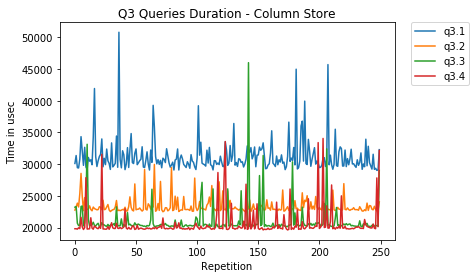
\includegraphics[width=0.49\textwidth]{images/q3-col.png}
	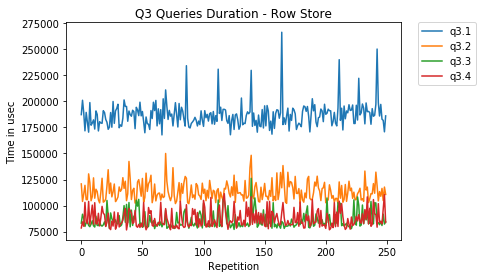
\includegraphics[width=0.49\textwidth]{images/q3-row.png}
	\caption{Q3 Vergleich Row vs Column}\label{auswertung:comp:q3}
\end{figure}

Aus \autoref{auswertung:comp:q3} lässt sich erkennen, dass Q3.1 sich relativ
zu Q3.2, Q3.3 und Q3.4 verbessert hat.
Um dies zu versehen werden im folgenden der Executionplan zu Q3.1 des Columnstores
und des Rowstores verglichen, welche in \autoref{auswertung:q3.1:col} und 
\autoref{auswertung:q3.1:row} im Anhang zu finden sind.
Beim Vergleich der Executionpläne wird deutlich dass der Columnstore dabei
einen Filter auf 4 Tabellen durchführt.
Dies ermöglicht eine Parallelisierung der Abfragen,
wohingegen beim Rowstore diese Parallelisierung nicht möglich ist.

\begin{figure}[H]
	\centering
	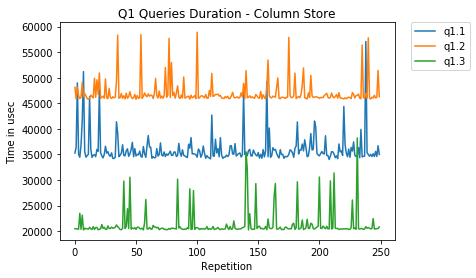
\includegraphics[width=0.49\textwidth]{images/q1-col.png}
	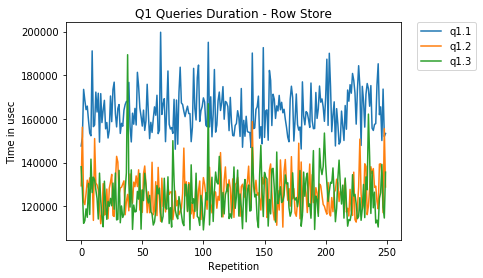
\includegraphics[width=0.49\textwidth]{images/q1-row.png}
	\caption{Q1 Vergleich Row vs Column}\label{auswertung:comp:q1}
\end{figure}

Interessant ist der Vergleich der Unterabfragen von Q1, da Q1.1
im Rowstore relativ zu Q1.2 langsamer ist, wohingegen im Columnstore
Q1.1 schneller als Q1.3 ist.
Vergleicht man die Executionpläne der Queries also Q.1.1 des Columnstores mit Q1.1 des Rowstores ist keine großer Unterschied zu erkennen, welcher diesen Effekt
erklären kann.
Analog dazu kann beim Vergleich des Executionplans von Q1.2 des Columnstores
mit dem Executionplan des Rowstores kein großer Unterschied erkannt werden.
Die Executionpläne sind im Anhang unter \autoref{exec:q1.1-col},
\autoref{exec:q1.2-col}, \autoref{exec:q1.1-row} und \autoref{exec:q1.2-row}
zu sehen.
Dementsprechend könnte der Effekt durch die interne Speicherverwaltung von HANA
beeinflusst werden.
Allerdings ist der Unterschied der Laufzeit beider Queries marginal.

Insgesamt kann Q3 im Rowstore besser ausgeführt werden,
da eine bessere Parallelisierung möglich ist.

\section{Vergleich der Query Execution Pläne - Query 4.3}
In diesem Abschnitt werden die Query Execution Pläne für den Row- und Columnstore der SQL Abfrage 4.3, dargestellt in \autoref{q42}, verglichen. Ein Grund dafür sind die großen Laufzeitunterschiede zwischen Row und Columnstore.
\begin{lstlisting}[label=q42, caption={Benchmark Query 4.3}]
select d_year, s_city, p_brand,sum(lo_revenue - lo_supplycost) as profit
from lineorder
join dim_date on lo_orderdatekey = d_datekey
join customer on lo_custkey = c_customerkey
join supplier on lo_suppkey = s_suppkey
join part on lo_partkey = p_partkey
where
s_nation = 'UNITED STATES'
and (d_year = 1997 or d_year = 1998)
and p_category = 'MFGR#14'
group by d_year, s_city, p_brand
order by d_year, s_city, p_brand;
\end{lstlisting}

\subsection{Query Execution Plan - Columnstore}
\autoref{qepCol} zeigt den Ablauf der Query Execution im Columnstore. Es ist zu erkennen, dass zu Beginn jede Tabelle einzeln nach den drei angegebenen Kriterien gefiltert wird.

\begin{figure}[H]
	\centering
	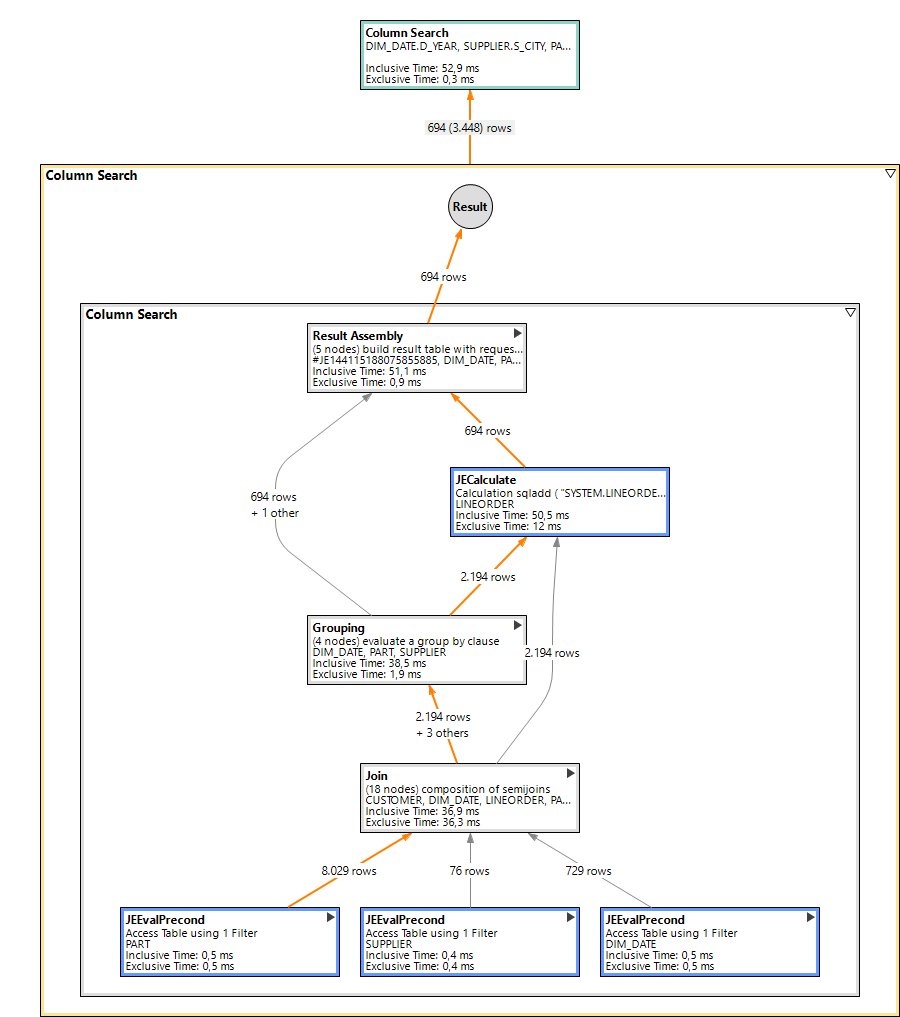
\includegraphics[scale=0.35]{images/col_q43_3}
	\caption{Query Execution Plan für Q4.3 - Columnstore \label{qepCol} }
\end{figure}

Die drei Tabellen liefern dann unterschiedlich große Ergebnismengen zurück:
\begin{itemize}
	\item Tabelle Part:			8029 Zeilen
	\item Tabelle SUPPLIER:		76 Zeilen
	\item Tabelle DIM\_DATE:	729 Zeilen
\end{itemize}
Die ermittelten Resultate werden dann in folgender Reihenfolge miteinander gejoint (vgl. \autoref{qepJoinCol}):
\begin{figure}
	\centering
	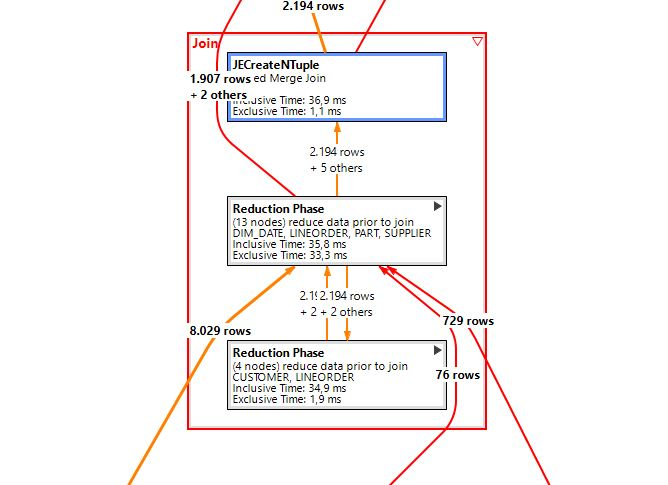
\includegraphics[scale=0.6]{images/colq43join}
	\caption{Join - Query Execution Plan für Q4.3 - Columnstore \label{qepJoinCol} }
\end{figure}
\begin{enumerate}
	\item Zuerst werden die beiden Tabellen \textbf{Lineorder} und \textbf{Customer} miteinander gejoint. In diesem Join fällt auf, dass auf keine der beiden Tabellen ein Filterkriterium angewendet wird und somit der Join unabhängig ausgeführt werden kann. 
	\item Sobald die Ergebnismengen der Tabellen \textbf{Part}, \textbf{Supplier} und \textbf{Dim\_Date} vorliegen, werden diese ebenfalls in einer \enquote{Reduction Phase} mit den Fremdschlüsseln der Tabelle \textbf{Lineorder} gejoint. 
	\item Wenn die ersten beide Schritte ausgeführt wurden, werden beide einzelnen Ergebnisse über einen Merge-Join in einer Ergebnismenge abgebildet und ausgegeben. 
\end{enumerate}
Anschließend an den Join wird eine Aggregation gebildet, die die Ergebnismenge nach Jahr, Nation und Produktkategorie gruppiert. Sobald die Gruppierung beendet ist, werden die Datensätze pro Gruppierung aufsteigend sortiert und anschließend ausgeben.


\subsection{Query Execution Plan - Rowstore}
\autoref{qepRow} zeigt den Query Execution Plan für das gleiche Query, nur dass die Daten im Rowstore abgelegt sind. Ohne genaueres Hinschauen fällt auf, dass die Ausführung sich im Vergleich zum Columnstore stärker an einem sequentiellen Ablauf orientiert.\\ Im Rowstore sieht die Reihenfolge der Abarbeitung des Joins wie folgt aus:
\begin{enumerate}
	\item Als erster Schritt wird ein Tablescan auf \textbf{Supplier} ausgeführt, der die Tabelle nach der Nation \enquote{UNITED STATES} filtert(76 Ergebnisse).
	\item Die Ergebnismenge wird mit der Tabelle \textbf{Lineorder} gejoint (228745 Ergebnisse)
	\item Bevor der Hash Join ausgeführt werden kann, wird ein Index Search auf die Tabelle \textbf{PART} ausgeführt, der die Produktkategorie eingrenzt. (8029 Ergebnisse)
	\item Es wird nun ein Hash Join auf mit den Ergebnisse der Schritte 1 und 2 mit den Ergebnissen des Schrittes 3 ausgeführt. Die Join wird über \textbf{LINEORDERS.LO\_Partkey} und \textbf{PART.P\_Partkey} ausgeführt. (9118 Ergebnisse)
	\item Zeitgleich zu dem Hash Join kann ein Table Scan auf die Tabelle \textbf{DIM\_Date} erstellet werden. (729 Ergebnisse).
	\item Anschließend werden die beiden Ergebnisse aus Schritt 4 und 5 wieder über eine Hash Join zu einem Ergebnis zusammengefasst. Dies geschieht über die Fremdschlüsselbeziehung der Tabelle \textbf{Lineorder} und \textbf{Dim\_Date} über die Spalte \enquote{LO\_Orderdatekey} bzw. \enquote{D\_Datekey}. (2194 Ergebnisse)
	\item Im letzten Join, dem Index Join, werden die zuvor in Schritt 6 ermittelten Ergebnisse mit der Tabelle \textbf{Customer} verknüpft. Dies geschieht über die Beziehung \enquote{Lineorder.LO\_Custkey = Customer.C\_Customerkey}. (2194 Ergebnisse)
\end{enumerate}
Nachdem alle Joins ausgeführt wurden, wird wieder eine Aggregation gebildet und die Gruppierung anschließend aufsteigend sortiert und das Ergebnis ausgegeben.
\begin{figure}[H]

	\centering
	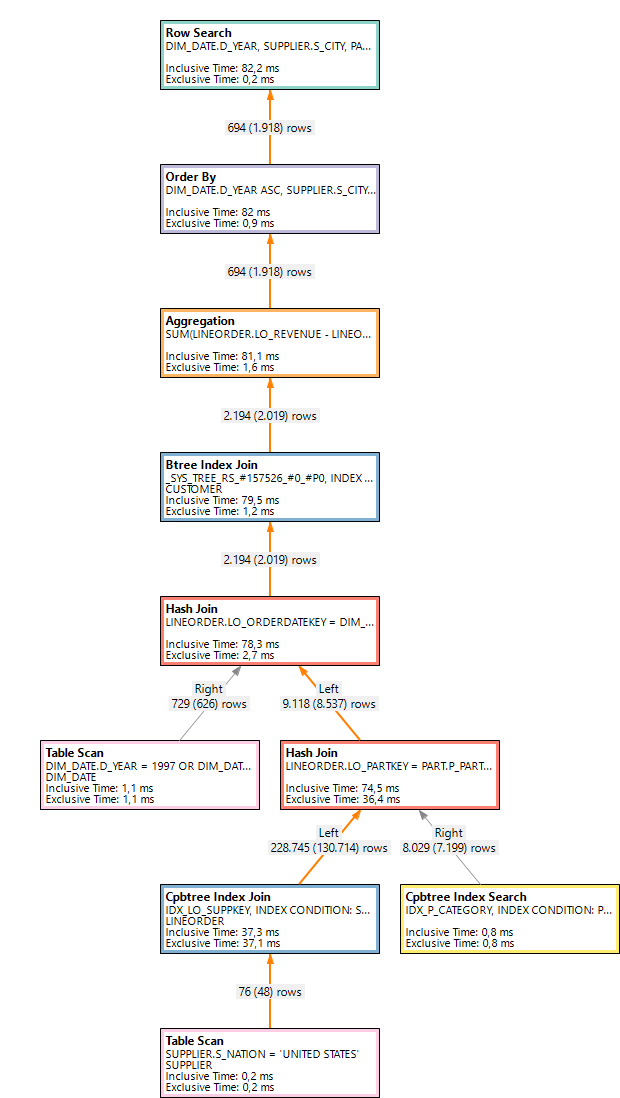
\includegraphics[scale=0.4]{images/row_q43}
	\caption{Query Execution Plan für Q4.3 - Rowstore 	\label{qepRow} }
\end{figure}

\subsection{Fazit Query Execution Plan}
Der große zeitliche Unterschied zwischen Row- und Columnstore lässt sich mit der sequentielle Ausführung des Query im Rowstore begründen. \\In beiden Ausführungen war ersichtlich, dass die Ausführung in die 3 Schritte, Filtern, Join und Gruppieren eingeordnet werden können. Allerdings sind im Rowstore das Filtern und Joinen eng miteinander verbunden und werden sogar abwechselnd nacheinander ausgeführt. Beim Columnstore hingegen war die Abgrenzung zwischen Filtern und Join deutlich stärker, da zuerst die Tabellen gefiltert wurden und anschließend die Ergebnismengen miteinander verknüpft.





\section{Einfluss der grundlegenden Indizes}\label{auswertung:basic_indizes}
%TODO
% Row with or without indices
% Column with or without indices

\subsection{Grundlegende Untersuchung für Columnstore}

\begin{table}[H]
\centering
    \begin{tabularx}{\textwidth}{lrrr}
        \toprule
        Merkmal             &   Col[ms]    &    Col Index[ms] & Abweichung[\%]\\
        \toprule
        Samples             &   250        &   250      &        \\
        \midrule    
        Median              &   752        &   574      & -23.6\%\\
        Average             &   755        &   578      & -23.4\%\\
        Total               &   188672     &   144605   & -23.3\%\\
        \bottomrule
    \end{tabularx}
\caption{Vergleich der Ergebnisse mit und ohne grundlegende Indizes für Columnstore.}
\label{tab:basic_index_col}
\end{table}

Durch hinzufügen der grundlegenden Indizes wurde der Benchmark
für Columstores sowohl im Schnitt als auch im Median schneller.
Im Schnitt wurde er 23,4\%, im Median um 23,6\% schneller.
Die Standardabweichung hat sich jedoch nur geringfügig verändert.
Die Werte streuen relativ gesehen also gleich stark wie zuvor.
Folglich konnten Mindest- und Maximallaufzeit auch deutlich reduziert werden. 

\iffalse
Diese Ergebnisse sind interessant,
da Columnstores bereits einen natürlichen Index
durch speichern der Daten in Spalten haben,
wie in \autoref{sec:col_store} beschrieben.
Deshalb profitieren Columnstore meist nicht von zusätzlichen Indizes.
\fi
Diese Ergebnisse sind interessant, da in der Regel davon ausgegangen wird, 
dass bei Columnstores kein großartiges Optimierungspotenzial durch Indizes vorhanden ist.
Um herauszufinden, warum trotzdem eine deutliche Verbesserung merkbar ist,
wird der Query-Execution Plan des Subqueries mit der deutlichsten Verbesserung
im folgenden untersucht.

\subsubsection{Untersuchung der Laufzeit für einzelne Query-Gruppen}

\begin{table}[H]
    \centering
    \begin{tabularx}{\linewidth}{crrr}
        \toprule
        Benchmarkgruppe & Col[ms]   & Col Index[ms] & Laufzeitreduzierung[ms|\%]\\
        \toprule
        Q1              & 104.7       & 68.5            & 36.2 | 34.5\%\\
        Q2              & 62.1        & 59.7            & 2.4 |  03.8\%\\
        Q3              & 96.2        & 54.8            & 41.4 | 40.8\%\\
        Q4              & 112.4       & 106.3           & 6.1 |  05.4\%\\
        \bottomrule
    \end{tabularx}
	\caption{Durchschnittslaufzeit für jede Benchmarkgruppe für Columnstore.}
\end{table}

Deutliche Verbesserungungen sind bei den Queries der Gruppen 1 und 3 festzustellen. Hier hat sich die Laufzeit um 35\% bzw. sogar 41\% reduziert. 
Die Queries dieser Gruppe werden im Detail untersucht, um geeignete Kandidaten für die Analyse des Execution-Plans zu finden.
Hier sind besonders bei Query 1.2 und 3.4 interessant, da diese die größte Verbesserung in ihrer Gruppe vorweisen können. 
Die Laufzeit wurde um 64\% für Query 1.1 und um mehr als 90\% für Query 3.4 reduziert. Woher diese Verbesserung kommen, soll im Folgenden durch die Analyse der Execution-Pläne von Query 1.1 und 3.4 geklärt werden.


\begin{table}[H]
    \centering
    \begin{tabularx}{\linewidth}{crrr}
        \toprule
        Benchmark           & Col[ms]       & Col Index[ms] & Laufzeitreduzierung[ms|\%]   \\
        \toprule
        Q1.1                & 36.1          & 36.4          & -0.3 | -0.8\%                \\
        Q1.2                & 47.8          & 16.8          & 31.0 | 64.8\%                 \\
        Q1.3                & 21.3          & 14.1          & 7.2 | 33.8\%                \\
        \midrule
        Q3.1                & 31.3          & 31.6          & -0.3 | -0.9\%                \\
        Q3.2                & 24.0          & 18.9          & 5.1 | 21.2\%                 \\
        Q3.3                & 21.3          & 2.1           & 19.2 | 90.1\%                \\
        Q3.4                & 20.5          & 1.6           & 18.9 | 92.1\%                \\
        \bottomrule
    \end{tabularx}
\caption{Durchschnittslaufzeit für Benchmarkgruppen 1 und 3 für Columnstore.}
\label{tab:q1_q3_col}
\end{table}

\subsubsection{Analyse des Query-Execution-Plans für Query 3.4}
\textbf{Hinweis:} Die Ergebnisse in diesem Abschnitt basieren auf Ausführung auf einem PC mit einer Intel Xeon 1230 V3 CPU mit 16GB DDR3 RAM. Die VM hatte 4 Kerne und 8GB RAM zur Verfügung.

Bei der Analyse des Query-Execution Plans zeigt sich schnell,
woher die große Geschwindigkeitssteigerung kommt.
Query 3.4 bildet einen Join von Lineorder auf Customer,
Supplier und Dim\_Date. 
Dieser Join erfolgt jeweils über den Fremdschlüssel in Lineorder.
Ohne Indizes ist dieser Join ausschlaggebend für die Laufzeit des Querys.
Durch anlegen von Indizes auf alle Fremdschlüssel,
kann der Join deutlich schneller ausgeführt werden.
Den größten Vorteil hat hier der Index auf LO\_Suppkey.

Der Execution Plan ohne Indizes ist in \autoref{execution-plan:before-index}, sowie \autoref{exec:q3.4-col-no}
zu finden und der Execution Plan mit Indizes ist in \autoref{execution-plan:after-index},sowie \autoref{exec:q34-col-index} zu finden.

Query 3.1 im Vergleich nutzt zwar auch Fremdschlüssel, um einen Join zu bilden,
allerdings sind hier die nicht indizierten Felder \verb+S_Region+, \verb+D_Year+,
\verb+C_Nation+ und \verb+S_Nation+ in der Where- und der Group by-Klausel gelistet,
wodurch eine Geschwindigkeitsverbesserung nicht möglich ist.

Auch bei Columnstores scheinen sinnvoll angelegte Indizes also einen deutlichen Unterschied zu machen.

\subsubsection{Analyse des Query-Execution-Plans für Query 1.2}
\textbf{Hinweis:} Die Ergebnisse in diesem Abschnitt basieren auf Ausführung auf einem PC mit einer Intel Xeon 1230 V3 CPU mit 16GB DDR3 RAM. Die VM hatte 4 Kerne und 8GB RAM zur Verfügung.
%https://archive.sap.com/discussions/thread/3429357


Bei Query 1.2 gibt es eine Besonderheit: Manchmal wird der Query über die OLAP-Engine ausgeführt\footnote{Um zu sehen, welche Engine verwendet wird, muss anstatt \enquote{Visualize Plan} die Option \enquote{Explain Plan} gewählt werden.}. 
Hierbei ist der Laufzeitunterschied zwischen Index und kein Index fast nicht mehr vorhanden, der Query mit Index braucht allerdings weniger Zeit zur Kompilation. 
Eigentlich ist die OLAP-Engine für \enquote{Analytical Views}, die im Star-Schema vorliegen,gedacht. Beim Star-Schema Benchmark liegen die Daten definitv im Start Schema vor.
Allerdings ist nicht klar, warum die OLAP-Engine manchmal verwendet wird und manchmal nicht. Ein Muster war hier nicht zu erkennen. 


\begin{wraptable}{r}{0.5\textwidth}
    \centering
    \begin{tabular}{lrr}
        \toprule
        Engine              & Col [ms]       & Col Index [ms]    \\
        \toprule
        OLAP                & 6           & 6         \\
        Colum               & 16          & 6         \\   
        \bottomrule
    \end{tabular}
	\caption{Durchschnittslaufzeit für Query 1.2 bei Columnstore.}
    \label{tab:olap_q12}
\end{wraptable}


%http://saphanatutorial.com/sap-hana-modeling/
%https://archive.sap.com/discussions/thread/3340726
Zunächst trat die OLAP-Engine nur auf, wenn Indizes hinzugefügt wurden, weshalb zunächst angenommen wurde, dass HANA an Hand der Indizes erkennt, dass es sich im Grunde um einen Analytical View handelt und dementsprechend optimiert.
Allerdings gab es auch Fälle, wo die OLAP-Engine auch ohne Indizes verwendet wurde. Kommt die OLAP-Engine zum Einsatz, so ist der Query in etwa so schnell, wie mit der Column-Engine in Kombination mit Indizes, siehe \autoref{tab:olap_q12}.

Kommt nicht die OLAP-Engine, sondern die \enquote{normale} Column-Engine zum Einsatz, so gibt es einen deutlichen Unterschied zwischen Index und kein Index. Hierbei kann der Index auf LO\_OrderDateKey für den JOIN genutzt werden und beschleunigt diesen somit.
Außerdem wird die Berechnung \textbf{sum(lo\_extendedprice*lo\_discount)} deutlich beschleunigt. Warum ist allerdings nicht klar, denn auf diese Felder wurde kein Index angelegt.


Schaut man sich genauer an, was an dieser Stelle passiert, so werden die gleichen Operationen auf die gleichen Datenmengen angewandt, allerdings sind die Operationen \textbf{mit} Index deutlich schneller.\footnote{Die letzte Zahl scheint jeweils die Laufzeit in ms zu sein, aber eine genaue Erklärung dieser Werte war leider nicht zu finden.}
\begin{lstlisting}[breaklines, caption=Ohne Index]
<executePop(
  <lockInputs(num=3,)=0.00>
    <calculateOnAttr(
      <calculateWithAggregation(rows=4301,inputs=2,outputs=1,)=8.04>
    rows=4301,outputs=1,)
  =8.15>
)=11.61>
\end{lstlisting}

\begin{lstlisting}[breaklines, caption=Mit Index]
<executePop(
  <lockInputs(num=3,)=0.00>
    <calculateOnAttr(
      <calculateWithAggregation(rows=4301,inputs=2,outputs=1,)=1.03>
    rows=4301,outputs=1,)
  =1.10>
)=1.18>
\end{lstlisting}

%https://www.stechies.com/important-hints-related-sap-hana/
\begin{wraptable}{r}{0.5\textwidth}
    \begin{tabular}{ccc}
        \toprule
        Engine              & No Index [ms]   & Index [ms] \\
        \toprule
        OLAP                & 187        & 188            \\
        Colum               & 296        & 226            \\   
        \bottomrule
    \end{tabular}
	\caption{Durchschnitt der Gesamtlaufzeit mit und ohne OLAP-Engine bei Columnstore.}
    \label{tab:olap}
\end{wraptable}



Wie in Tabelle \ref{tab:olap} zu sehen, ist die OLAP-Engine insgesamt sowohl mit, als auch ohne Index deutlich schneller, als die Column-Engine. 

Durch den HINT \enquote{USE\_OLAP\_PLAN} kann die OLAP-Engine als bevorzugte Engine festgelegt werden. Führt man jeden der Querys mit diesem Hint durch, so liefert dies die folgenden Ergebnisse:

\begin{figure}[H]
    \centering
    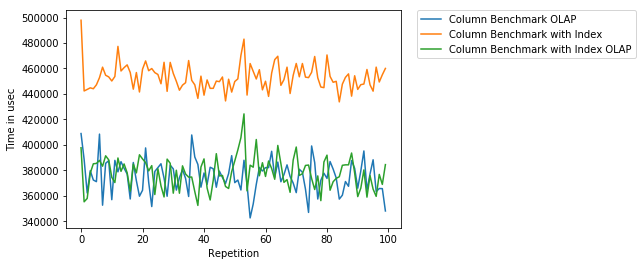
\includegraphics[scale=0.7]{images/olap_column_overall.png}
    \caption{Vergleich der Gesamtlaufzeit für Columnstore mit Indizes, testweise mit OLAP-Hint. n=100}
	\label{fig:olap_column_overall}
\end{figure}

Wie in Grafik \ref{fig:olap_column_overall} zu sehen, wird durch den OLAP-Hint eine deutliche Beschleunigung erzielt. Ob zusätzlich noch ein Index existiert hat jedoch wenig bis keinen Einfluss.

Bei genauerer Betrachtung der Laufzeit pro Benchmarkgruppe fällt besonders auf, dass die Querys der Gruppe 1 nicht von der OLAP-Engine profitieren, sondern sogar langsamer werden. 
Warum dies beim Durchführen des Benchmarks, aber nicht bei Analyse der Execution-Pläne der Fall ist, ist nicht klar.

\iffalse
\begin{figure}[H] 
    \centering{
    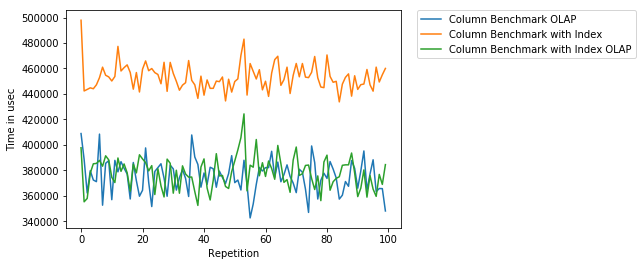
\includegraphics[scale=0.7]{images/olap_column_overall.png}
    \caption{Vergleich der Gesamtlaufzeit für Columnstore mit Indizes, testweise mit OLAP-Hint. n=100}\label{fig:olap_column_overall}}
\end{figure}
\fi

Die anderen Benchmarkgruppen werden durch den OLAP-Hint jedoch schneller, Gruppe 3 und 4 nur geringfügig, Gruppe 2 jedoch wird nahezu doppelt so schnell.
\begin{table}[H]
    \centering
    \begin{tabularx}{\textwidth}{lXrrrr}
    \toprule
	Wert        &	OLAP-Hint & Q1 	    &	Q2 	    &	Q3	    &	Q4 \\
    \toprule
    Average	    & Nein        &	23.5	&	72.5	&	60.4	&	69.9 \\
    Average     & Ja	      &	26.3	&	36.4	&	58.3	&	65.6 \\
    \midrule
    Median	    & Nein        &	23.4	&	72.1	&	60.2	&	69.3 \\
    Median	    & Ja          &	26.5	&	36.0	&	59.5	&	66.0 \\
    \bottomrule
    \end{tabularx}
	\caption{Laufzeit jeder Benchmarkgruppe für Columnstore mit Index, testweise mit OLAP-Hint. n=100}
    \label{tab:olap_bench}
\end{table}
%Hier dann Tabelle, wenn Benchmark fertig ist. 

\subsubsection{Fazit für Columnstores}
Auch Columnstores können durch geschickt gewählte Indizes deutlich beschleunigt werden. Durch Nutzung der OLAP-Engine können diese Beschleunigungen jedoch nochmals teils deutlich überboten werden. 
Es erscheint sinnvoller, sein Augenmerk darauf zu legen, dass Querys diese auch nutzen. Dies ist zwar über einen HINT möglich, davon wird in der Praxis jedoch abgeraten.
%https://archive.sap.com/discussions/thread/3277920

\subsection{Grundlegende Untersuchung für Rowstore}

\begin{table}[H]
    \begin{tabularx}{\textwidth}{lrrr}
        \toprule
        Wert                & Row[ms] & Row Index[ms]   & Abweichung [\%]\\
        \toprule
        Samples             & 250      & 250            &       \\
        \midrule
        Median              & 3519     & 3006           &  14.5\%     \\
        Average             & 3539     & 3048           &  13.8\%     \\
        Total               & 884960   & 762128         &       \\ 
        \bottomrule
    \end{tabularx}
\caption{Vergleich der Ergebnisse mit und ohne grundlegende Indizes für Rowstore.}
\label{tab:basic_index_row}
\end{table}





\begin{table}[H]
    \begin{tabularx}{\textwidth}{lrrr}
        \toprule
        Wert                & Row[ms] & Row Index[ms]   & Abweichung [\%]\\
        \toprule
        Samples             & 250     &  250            &       \\
        \midrule
        Median              & 3426    &  2877           &       \\
        Average             & 3440    &  2881           &       \\
        \bottomrule
    \end{tabularx}
\caption{Vergleich der Ergebnisse mit und ohne grundlegende Indizes für Rowstore.}
\label{tab:basic_index_row}
\end{table}

\begin{table}[H]
    \begin{tabularx}{\linewidth}{lrrrrrr}
        \toprule
                &   q1.1    &   q1.2&	q1.3&	q2.1&	q2.2&	q2.3 \\
        \toprule
        Row[ms]	        &	163	    &	133	&	127	&	139	&	111	&	102  \\
        Row Index[ms]   &   156     &   13	&   3	&   73	&   16	&   4    \\
        Abweichung[ms]  &   7       &   120 &   124 &   66  &   95  &   98   \\
        Abweichung[\%]  &   4.2     &   90.2&   97.6&   47.4&   85.5&   96.0 \\    
\bottomrule
\end{tabularx}
\caption{Vergleich der Ergebnisse mit und ohne grundlegende Indizes für Rowstore.}
\label{tab:basic_index_row}
\end{table}
\section{Auswirkung unterschiedlicher Hardwarekonfiguration}\label{auswertung:hardware}

Nicht nur die Betrachtung unterschiedlicher Konfigurationen auf Software-Ebene ist interessant, sondern auch die auf simulierter Hardware-Ebene. Die eingesetzten Hardwarekonstellationen wurden im Kapitel zur Ausführung des Benchmarks beschrieben und werden nun miteinander verglichen. Zum Einsatz kommen die Ergebnisse des Analysers, welche als Visualisierungen sowie Aggregaten-Werten präsentiert werden. In der Analyse werden wird zuerst auf den Columnstore eingegangen und anschließend vergleichend auf den Rowstore. 

\subsection{Columnstore}

\begin{figure}[H]
    \centering{
    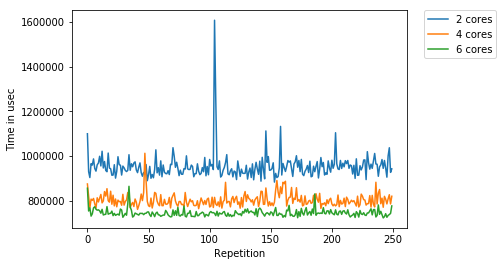
\includegraphics[scale=0.7]{images/colcpu.png}
    \caption{Benchmark im Columnstore unter Variation der CPU Kerne}\label{colcpu}}
\end{figure}


\autoref{colcpu} zeigt die Ausführungsdauer über den 250 Durchläufen des Benchmarks bei konstanten 8 Gigabyte RAM. Generell bewegt sich die Ausführungsdauer pro Benchmark hauptsächlich im Bereich von ca. 0.7 Sekunden bis 1 Sekunde. Dabei werden die schnelleren Werte, wie erwartet, durch den sechs-Kerner gebildet und die langsameren Werte durch den zwei-Kerner. Werden der sechs-Kerner(0.75 Sekunden) und der zwei-Kerner(0.95 Sekunden) anhand ihren arithmetischen Mitteln miteinander verglichen so ergibt sich eine prozentuale Differenz von 26.7\%. Der vier-Kerner hingegen erreicht eine durchschnittliche Ausführungszeit von 0,8 Sekunden was ihm eine Differenz von 7\% im Vergleich zum sechs-Kerner einbringt. 
Grundsätzlich gilt, dass im Columnstore im HANA Umfeld dank der begünstigten Parallelisierung eine bessere Ausnutzung der CPU durch mehrere Threads stattfindet. Dadurch wird die Nutzung der Hardware optimiert und eine bestmögliche Performance wird erzielt. Pro zusätzlichem Kern kann die Ausführungszeit halbiert werden, indem die Last gleichmäßig auf die Kerne aufgeteilt wird. Diese Überlegung stimmt mit den Messwerten überein und es lässt sich auf einen quadratischen Zuwachs der Ausführungszeit abhängig zur Anzahl der CPU-Kerne schliessen. 

\begin{figure}[H]
    \centering{
    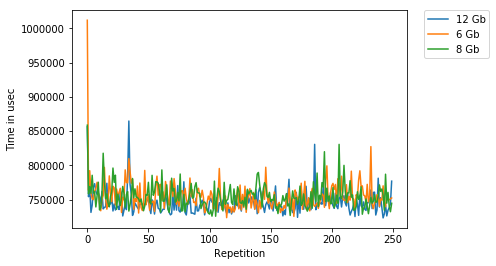
\includegraphics[scale=0.7]{images/colram.png}
    \caption{Benchmark im Columnstore unter Variation des RAMs}\label{colram}}
\end{figure}

\autoref{colram} zeigt die Ausführungsdauer über den 250 Durchläufen des Benchmarks bei konstanten 6 CPU Kernen. Die Ausführungsdauer pro Benchmark scheint nicht markant zu variieren, auch wenn die genauere Betrachtung der Aggregat-Werte zeigt, dass der Benchmark unter 12 Gigabyte RAM im Schnitt um eine Hunderdstel Sekunde schneller ist, als bei 6 und 8 Gigabyte. Ein besseres Mittel zum Vergleich als die Durchschnittslaufzeit bildet in diesem Falle die Standardabweichung der Laufzeiten, welche ein Maß für die Stabilität des Benchmarks darstellt. Diese beträgt bei 12 Gigabyte RAM gerade einmal 16 Millisekunden, während sich bei 8 Gigabyte ein 4 prozentiger Zuwachs und bei 6 Gigabyte ein 37 prozentiger Zuwachs erkennen lässt. Daraus lässt sich ableiten, dass die Stabilität stark unter der Einschränkung des RAMs leidet, und somit einzelne Anfragen erheblich länger dauern können. Vermutlich liegt die Unregelmäßigkeit vorallem darin begründet, dass bei reduziertem RAM externe Faktoren (Cache-Miss, Zugriffszeit) deutlicher zum tragen kommen. 

\subsection{Rowstore}

\begin{figure}[H]
    \centering{
    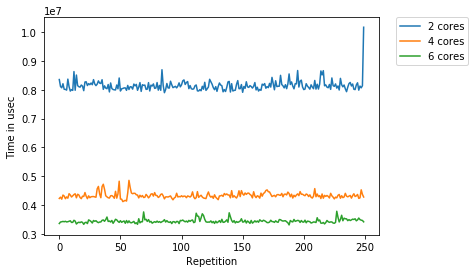
\includegraphics[scale=0.7]{images/rowcpu.png}
    \caption{Benchmark im Rowstore unter Variation der CPU Kerne}\label{rowcpu}}
\end{figure}

\autoref{rowcpu} zeigt die Ausführungsdauer über den 250 Durchläufen des Benchmarks bei konstanten 8 Gigabyte RAM. Zu erkennen ist die starke Abweichung der Ausführungszeiten, welcher deutlicher ausfällt als im Columnstore. Der zwei-Kerner liegt mit einer durschnittlichen Ausführungszeit von 8,2 Sekunden 137\% über der Ausführungszeit des acht-Kerners, welcher nur 3,4 Sekunden im Schnitt braucht. Die Abweichung des sechs-Kerners beträgt dagegen nur 26\%. 
Es scheint als würde die Anzahl der CPU-Kerne einen größeren Einfluss haben im Rowstore als im Columnstore. Eine mögliche Erklärung dafür kann folgendermaßen aussehen: 
Da die Daten im Columnstore blockweise gelesen werden können, haben die Lesezugriffe eine längere Ausführungszeit, da auch viele Daten in einem Zuge gelesen werden können. Der komplette Satz an Daten wird anschliessend von der CPU ausgewertet, wobei die Auswertung kürzer dauert als der Speicherzugriff. Dadurch wird das RAM zum Bottleneck und die CPU unrelevanter für die Ausführungszeit. 
Im Rowstore müssen viele einzelne Lesezugriffe durchgeführt werden, wobei die einzelnen Daten direkt verarbeitet werden von der CPU. Die Parallelität ist nicht in dem Maße gegeben wie im Columnstore, wodurch stets das RAM auf die CPU wartet und umgekehrt. Daraus ensteht eine erhöhte Relevanz der CPU für die Ausführungszeit als beim Columnstore. 

\begin{figure}[H]
    \centering{
    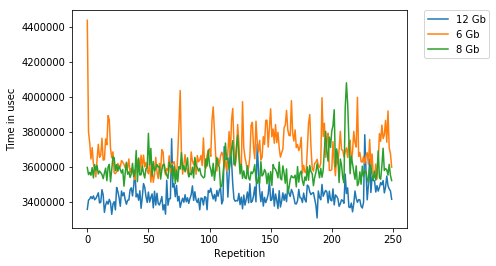
\includegraphics[scale=0.7]{images/rowram.png}
    \caption{Benchmark im Rowstore unter Variation des RAMs}\label{rowram}}
\end{figure}

\autoref{rowram} zeigt die Ausführungsdauer über den 250 Durchläufen des Benchmarks bei konstanten 6 CPU Kernen. Die Ausführungszeiten unterscheiden sich ebenfalls deutlicher als beim Columnstore. Unterschieden sich im Columstore die durchschnittlichen Ausführungszeiten von 12 Gigabyte und 6 Gigabyte RAM noch um 1,33\%, so liegt der Unterschied nun bereits bei 7,13\%. Die Standardabweichungen scheinen dasselbe Muster wie im Columnstore aufzuweisen: Je mehr RAM, desto stabiler läuft der Benchmark. Im Falle des 6 Gigabyte Systems sind enorme Ausschläge zu beobachten, obwohl teilweise sogar die Ausführungszeit des 8 Gigabyte Systems unterboten wird. 
Die erhöhte Relevanz der Menge an verfügbarem RAM scheint im Rowstore ebenfalls von größerer Bedeutung für die Laufzeit zu sein als im Columnstore. Während im Columnstore automatisch Optimierungen, wie Indexierung und Kompression stattfinden, können diese im Rowstore womöglich nur bei ausreichend RAM durchgeführt werden. 

